\documentclass[11pt]{article}

\usepackage[letterpaper]{geometry}
\usepackage{amsmath}
\usepackage{amsthm}
\usepackage{amssymb}
%\usepackage[utf8]{inputenc}
\setcounter{secnumdepth}{3}
\usepackage{url}
\newcommand{\reals}{{\mathbb R}}
\usepackage{wrapfig}
\usepackage{graphicx}
\usepackage{subfigure}
\setlength{\textheight}{8.75 in}
\setlength{\topmargin}{-0.75 in}
\graphicspath{ {img/}}

\title{An Improved Approximation Algorithm for Multiway Cut\\Gruia Calinescu Howard Karloff Yuval Rabani\\Final report for CS 6150}
\author{Gurupragaash Annasamy Mani \and Praveen Thiraviya Rathinam}

\begin{document}
\maketitle

\section{Multiway Cut}

Consider an undirected graph G = (V, E) with vertices V = $\{1, 2, $\dots$, n\}$ and edges E with weights w: E $\rightarrow R^{+}$. Let T = $\{1, 2, . . . , k\} \subseteq$ V be a set of terminals. Multiway Cut is the problem of finding a minimum cost cut C $\subseteq$ E such that no connected component of G(V, E - C) contains two terminals from T. In case of just two terminals, minimum multiway cut is just a min s-t cut problem and hence can be solved in polynomial time by running a maximum flow algorithm from one terminal to the other. But when the number of terminals becomes $\ge 3$, then the problem of computing the minimum weight multiway cut is NP-hard and max SNP-hard even for fixed $k \ge 3$ by Dahlhaus, Johnson, Papadimitriou, Seymour and Yannakakis. In other words, there is a constant $\delta >$ 1 such that it is NP-Hard to even approximate the solution to within a ratio of less than $\delta$. Unless P = NP, there is no polynomial-time approximation scheme for Multiway Cut.
\paragraph{APX-Hard/SNP-Hard}
APX(Approximable) class is a set of NP optimization problems in which algorithms can be used to find an answer within some fixed multiplicative factor of the optimal answer. APX class is also known as MAX-SNP. A problem is said to be SNP-hard if it does not have a Polynomial Time Approximation Scheme(PTAS).
 
\section{Previous Work on Multiway Cut} 
\subsection{Isolation Heuristic}

Dahlhaus et al.\cite{Dahlhaus} initiated the study of multiway cut problems. They proposed a simple combinatorial isolation heuristic to approximate the solution to these kinds of problems.In isolation heuristic, given a undirected weighted graph G = (V,E) and K terminals, in each iteration we attach one terminal to the source and all the other terminals to the sink and then run a max-flow algorithm and find the min-cut for each turn. Let the edge set after each iteration be $E_i$. Now the lowest k-1 cuts are taken and the union of them gives the multi-way cut. This algorithm gives an approximation of $2(1-\frac{1}{k})$.\\\\
\textbf{Proof:}
\begin{itemize}
    \item Run the isolation heuristic scheme and get the set of edges. Let they be A.
    \item Let $E^*$ be the optimal edge set for the multiway cut with K terminals. Then it means if $E^*$ is removed then there will be $K$ disjoint connected graphs ($V_1, V_2,\cdots,V_k$), each having one terminal respectively.
    \item $E^* = \sum_{i=1}^{k}{E_i^*}$ and each $E_i^*$ represents the edges removed to disconnect $V_i$ from rest.
    \item Let $\delta(V_i)$ denote the set of all outgoing edges from $V_i$.
    \item Now we can say that, $w(E_i) \le w(\delta(V_i))$ because both isolate the terminal $i$ from the rest and we know $E_i$ is the mincut. So $w(E_i)$ cannot be greater than $w(\delta(V_i))$
    \item $2w(E^*) = \sum_{i=1}^{k}{\delta(V_i)} $. It is 2 times since each edge is double counted in the process(If there is a edge between $i$ and $j$, then both $\delta(V_i)$ and $\delta(V_{i+1})$ will include that edges).
    \item We know $w(A) \le (1 -\frac{1}{k})(\sum_{i=1}^k w(E_i^*))$. This is because, A is union of first K-1 smallest set. In this expression, we are adding up all the $K$ values. Since only $k-1$ values are taken, we are multiplying it with $1 - \frac{1}{k}$ and since it the union of all these set, it will be equal to or less than the summation of indiviual sets.
        \begin{align*}
            w(A) &\le (1 -\frac{1}{k})(\sum_{i=1}^k w(E_i^*)) \\
            &\le (1 -\frac{1}{k})(\sum_{i=1}^k w{\delta(V_i)}\\
            &\le 2(1 -\frac{1}{k})w(E^*)\\
          w(A)  &\le 2(1 -\frac{1}{k}) OPT
        \end{align*}
\end{itemize}
\subsubsection{Alon's Improvement}
Noga Alon~\cite{Dahlhaus_Alon} observed that for the special cases of k = 4 and k = 8 improvements can be obtained using a variant of the isolation heuristic. For k = 4, the Isolation Heuristic provides a guarantee of 3/2. An improved guarantee of 4/3 can be obtained as follows: For each partition of the terminals into sets $S_1$,$S_2$ of size two, use max flow techniques to
compute the minimum cut that separates the terminals in $S_1$ from those in $S2$. Output the union of the two best such cuts. The reader can readily verify that this union is a 4-way cut whose weight is at most 4/3 optimal. This approach requires only three max flow computations versus the four needed by the Isolation Heuristic, so it is faster as well.For k = 8, the guarantee of our theorem can be improved from 7/4 to 12/7. Unfortunately, the above approach did not yield improvements over the Isolation Heuristic for any values of k other than 4 and 8.

\subsection{Greedy Split Algorithm}
There is another greedy algorithm technique that can be used to solve the multiway cut problem. 
This algorithm also has an approximation ratio of $2 - \frac{2}{k}$. The algorithm is as follows:
\begin{itemize} \itemsep -3pt
\item Find the cheapest cut that splits G into 2 components such that each contains atleast a  terminal
\item Find the cheapest cut dividing the 2 components such that each of the 3 components contains atleast a  terminal
\item Find the cheapest cut dividing the 3 components such that each of the 4 components contains atleast a terminal
\item The steps are repeated until each of the k components contains a terminal. At each step, the algorithm chooses the cheapest cut among all components.
\end{itemize}

\subsection{Polyhedral Approach}
Chopra et al.\cite{chopra_1,chopra_2} and Cunningham\cite{cunningham} investigated on solving multiway cut problem using a polyhedral approach.But these two approaches too had an approximation ratio of $2(1 - \frac{1}{k})$.

\textbf{Chopra et al.} proposed an integer formulation and studied the associated polyhedron. They further proposed an extended formulation  which was tighter than all known solution at that time and also observed that when the underlying graph is a tree, the multiway cut problem can be solved in linear time by a straightforward dynamic programming algorithm.

\textbf{Cunningham} showed that for one particular formulation of the problem, the value of the minimum multiway cut is almost twice of its linear relaxation.

\subsection{Non-linear Formulation}
Bertsimas et al.\cite{Bertsimas} proposed a non-linear formulation of the multiway cut. Here the optimal solution formulated was an integral one. They suggested several polynomial time-solvable relaxations and gave a simple randomized rounding argument yielding the same approximation ratio of $2(1 - \frac{1}{k})$

\section{Overview of the solution and the Basic Notations}
\subsection{Overview}
 Authors use a geometric relaxation of the k-way cut which uses a $(k-1)$ simplex $\bigtriangleup$ which has k vertices and the $i^{th}$ vertex is point x in $\bigtriangleup$ with $x_i$ = 1 and all other coordinates 0. Relaxation is as follows: Map the nodes of the graph to points in the simplex such that the i terminals are mapped to the $i^{th}$ vertex. Each edge is mapped to the line between its end points. The goal here is to minimize the volume of G. The embedding is a relaxation of the minimum k-way cut problem. Once the basic premises are set, the authors find the minimum volume embedding through linear programming. They then propose a randomized rounding scheme to extract the multiway cut which induces a k-way cut in the embedded graph and separates the graph into k isolated components. This cut is supposed to have a cost at most $1.5 - \frac{1}{k}$ times the volume of the embedding. We discuss about the proposed solution in detail in the sections below. 

\subsection{Simplex Solution}
A simplex is a generalization of the notion of a convex polyhedron to arbitrary dimensions. In our case, we solve the linear programs using the simplex formulation. A $k$ dimension simplex has $k + 1$ vertices. Linear programs can be solved using the simplex approach.Linear program operates on simplicial cones, and these become proper simplices with an additional constraint. The simplicial cones in question are the corners (i.e., the neighborhoods of the vertices) of a geometric object called a polytope. The shape of this polytope is defined by the constraints applied to the objective function. For solving the multiway cut, we keep the k terminals as vertices and develop a $k-1$ dimensional convex polytope given by $\{x \in {\mathbb R}^k \vert \ (x \ge 0) \wedge (\sum_i x_i = 1) \}$

\subsection{L1 Norm}
L1-norm is also known as Mean-Absolute Error(MAE) or Sum of Absolute Difference(SAD). It is basically used to find the sum of the all the value of a variable. L1 norm of x is basically denoted by $\vert\vert x \vert\vert$. It can also be used to find the difference between two vectors
\begin{align*}
\text{SAD}(x_1, x_2) = \vert \vert x_1 - x_2 \vert \vert = \sum \vert x_1 - x_2 \vert
\end{align*}

\subsection{Unit Vector}
Unit vectors are used for denoting the spatial direction and generally represent the axes of a cartesian co-ordinate system. In our case, the unit vectors are used to represent the position of the vertices of the graph on the $k-1$ dimensional simplex. For j = 1, 2,$\dots$,k, $e^j \in \mathbb{R}$ denotes the unit vector given by $(e^j)_j$ = 1 and $(e^j)_i$ = 0 for all i $\notin$ j.

\subsection{Semimetric}
Semimetric is a pair $(V, d)$, where $V$ is a set and $d$ is a function which operates on $V$ such that $d: V \times V \rightarrow \mathbb{R}$, $\forall u,v \in V$.
\begin{align*}
d(u, v) &= d(v, u) \ge 0\\
d(u, u) &= 0\\
d(u,v) &\le d(u,w) + d(w,v) 
\end{align*}

\section{Linear Programming  Relaxations}
\subsection{LP1 and LP2}
\begin{align*}
\text{Minimize} \qquad  \sum\limits_{uv \in E}{c(u, v) \ d(u, v)} \ \text{is the objective function}
\end{align*}
\vspace{-20pt}
\begin{align}    
\text{such that} \ \qquad & (V,d) \text{ is a semimetric}\\
&d(t_1, t_2) = 1 \quad \forall t_1, t_2 \in T, t_1 \neq t_2\\
&d(u, v) \in (0,1) \forall u, v \in V
\end{align}
\begin{figure}

\subfigure[Sample Graph]{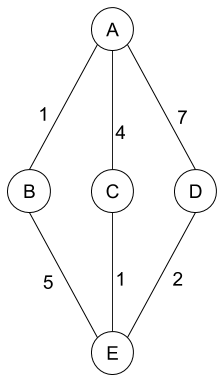
\includegraphics[scale = 0.25,width = 0.35\textwidth]{graph}}
\hfill
\subfigure[Sample Graph 2]{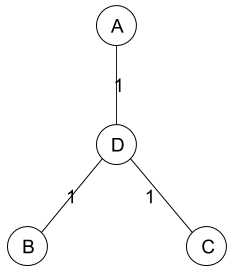
\includegraphics[scale = 0.25,width = 0.35\textwidth]{graph2}}
\caption{Graphs to explain the LP constraints}
\label{fig:sample_graph}
\end{figure}
Consider the graph in Figure~\ref{fig:sample_graph}(a). Let nodes A and E be terminals and we want to find a cut. In the LP, all the $d(u,v)$ where $uv$ is an valid edges is the decision variable and the value of it can be 0 or 1. From equation 3, we can say that $d(A, E) = 1$ and there are not anymore straight forward constraints. But from the semimetric property, we can write $d(A, E) \le d(A, B) + d(B, E)$, $d(A, E) \le d(A, C) + d(C, E)$ and $d(A, E) \le d(A, D) + d(B, D)$. Now the LP should assign atleast value 1 to one of the pairs in $(d(A, B), d(B, E))$, $d(A, C), d(C, E)$ and $d(A, D), d(B, D)$. Assigning (u, v) with a value 1 means, selecting the edge for the cut. Since our objective function is to minimize it, the LP will find which edge costs minimum and that will be the optimal solution. The authors come up with much more stricter constraints to reduce the number of valid solution.
\begin{align}
\sum\limits_{t \in T}{d(u, t)} &= k - 1 \quad \forall u \in V\\
d(u, v) &\ge \sum\limits_{t \in S}{[d(u, t) - d(v, t)]}
\end{align}
 Lets look into the constraint $\sum\limits_{t \in T}{d(u, t)} = k - 1 \quad \forall u \in V$ using the example Figure~\ref{fig:sample_graph}(b). In this example, the nodes A, B and C are terminals. If we run our LP without the new constraints, there are four valid solutions, which represent the cuts {(AD, DB), (AD, DC), (DB, DC) and (AD, DB, DC)}. In this set of values, (AD, DB, DC) is not a optimal one but still is a valid solution. In a large graph, there could be many such solutions, but can be removed easily with the new constraint, $\sum\limits_{t \in T}{d(u, t)} = k - 1 \quad \forall u \in V$. The new constraint says, if there is a node u, as long as its not connected to more than one terminal it is fine. So if there are k nodes, then $\sum\limits_{t \in T}{d(u, t)} = k - 1$, which means only $K-1$ cuts are required and not $K$ cuts. Similarly they add one more constraint $d(u, v) \ge \sum\limits_{t \in S}{[d(u, t) - d(v, t)]}$. Here $S$ is a subset of the terminal set $T$. When $S = T$, the expression has the maximum value which is greater than 0. These two constrains constitute LP2.

\subsection{Successive Linear Programming}
Successive Linear Programming(SLP) is an optimization technique for solving non-linear optimization problems. 

\begin{itemize} \itemsep -3pt
    \item As discussed earlier, any valid solution will split the Graph $G(V,E)$ into $K$ graphs ($C_1, C_2,\cdots,C_k$), with each $C_i$ having a terminal $S_i$
    \item Let $\delta(C_i)$ represent the set of edges which goes out of $C_i$
    \item Each vertex $v \in V$ is represented as $x_i^j$ and this value is set to 1 if the $i^{th}$ vertex is part of the component $C_i$, else its set to 0. Since a vertex can be a part of only one component, we can say that $\sum_{j=1}^{k}{x^j} = 1, \forall x \in V$, 
    \item We define another notation $z_e^i$ which operates on all the edges in E and is set to 1 if the edge $e$ is in $\delta(C_i)$ else its set to 0
    \item If $e$ is in the $\delta(C_i)$, then it connect $(u,v)$ where $u \in C_i, v \notin C_i$. Thus we can write $z_e^i$ as $z_e^i = x_u^i - x_v^i$, since $x_u^i$ will be 1 and $x_v^i$ will be 0, as per the definition of $x$. If $e$ is not in the $\delta(C_i)$, then both u and v belong to a same component, then both $x_u^i$ and $x_v^i$ will be 1 if both belong to component $C_i$ else both will be 0.
    \item Now for the objective function is $\frac{1}{2}\sum\limits_{e \in E}{c_e * \sum\limits_{i=1}^{k}{z_e^i}}$, where $c_e$ is the cost/weight of the edge. We are multiplying it with $\frac{1}{2}$ because of the double counting which we discussed in the previous explanation.
\begin{align*}
\text{Minimize} \qquad & \frac{1}{2}\sum\limits_{e \in E}{c_e * \sum\limits_{i=1}^{k}{z_e^i}}\\
\text{such that}  \qquad z_e^i &= |x_u^i - x_v^i|, \quad \forall e \in E\\
\sum\limits_{i=1}^{k}{x_v^i} &= 1,\quad \forall v \in V\\
x_{s_i}^i &= 1,\quad \forall s_i \in T \ \text{(Set of Terminals)}\\
x_v^j &\ge 0, \quad \forall v \in V \ (\text{Got by adding LP relaxation to }x_v^j \in (0,1),\ \forall v \in V)
\end{align*}
\end{itemize}

  \paragraph{Proposition 1} Authors state that LP2 and SLP are equivalent. They prove this either by using Case 1 or Case 2 as stated below.  
  \begin{enumerate} \itemsep -3pt
  \item   Assuming a feasible solution for LP2 and then computing a solution for SLP which will be of similar value
  \item Assuming a feasible solution for the SLP and then computing a solution for the LP2. For the first
  \end{enumerate}
In the first case, using the solution for LP2, it is proven that all the nodes in the graph lie in the simplex and the distance between the vertices and the terminals is less than the distance between those vertices as stated in constraint 5. In the second case, assuming d(u,v) = $\frac{1}{2} \vert \vert x^{u} - x^{v} \vert \vert$, we can compute the solution for LP2. Through these proofs, the authors state that objective function in case of LP2 and SLP are equivalent and feasible.
  
\section{Subdivisions}
Lets say we have a graph $G(V,E)$ with $K$ terminals and $c(u,v)$ representing the cost of the edge connecting nodes(u,v). We can create a graph $G^{'}$ from G, by splitting the edges across $(u,v)$, into two edges by introducing a node. The new edges are $(u,w)$ and $(w,v)$ and $w$ is a new node which is a normal node and not a terminal. Now we assign $c(u,v)$ to both $c(u,w)$, $c(w,v)$ and the edge $(u,v)$ is removed. We do this process some finite number of times and now we have a graph $G'(V',E')$  which is constructed from $G(V,E)$. The authors claim that if G' has a multiway cut $C^{'}$ of cost Z, then we can construct a cut C for G which has a cost atmost Z. We can do this by looking into the edge in $C^{'}$. $\forall e' \in C'$ check if $e' \in E$, then add it to C. If $e' \notin E$, find the edge $e \ \text{in} \ E$ which was split to get $e' \in E'$ and add $e$ to C. This set C is the multiway cut for graph G.

\subsection{Purpose of subdivisions}
For the algorithm proposed in the paper to work, the nodes in the graph should have the property that the unit vectors of the nodes must differ by only 0 or 2 co-ordinates. But the graphs normally do not have this property. We induce this property into the graph with the help of subdivision method. As explained previously, we split the edges till the unit vectors of all the nodes in the graph differ by atmost 2. This process of subdivision, can lead upto $k$ divisions for each edge and thereby introducing a max of $k\vert E \vert$ nodes in the graph. If we run the algorithm in the graph now, we will can get a solution which is $(1.5 - \frac{1}{k})OPT$. This is what is discussed in \textbf{Proposition 2} and \textbf{Lemma 3} in the paper. 

\section{Randomized Rounding Algorithm}
Randomized rounding is a technique for designing and analyzing approximation problems. The basic idea is to use a probabilistic method to convert an optimal solution of a relaxation of the problem into an approximately optimal solution to the original problem.It has three steps:
\begin{enumerate} \itemsep -3pt
\item Converting the original problem into a integer linear program(ILP).
\item Calculate optimal fractional solution $x$ to the linear programming relaxation of  ILP
\item Rounding the fractional solution $x$ of the LP to the integer solution $x^{'}$ of ILP 
\end{enumerate}

The multiway cut problem can be converted into an integer program through the linear programming relaxations mentioned in the previous section. Next the authors propose a randomized rounding algorithm to find the multiway cut with cost within a factor of $1.5 - \frac{1}{k}$ of the optimal solution. Take an optimal solution to the relaxation with edges whose endpoints differ in at most two coordinates, and let OPT denote its cost. Once we find the multiway cut of expected cost, we can use lemma 2 and proposition 3 and extend it to general cases.\\
\vspace{-10pt}
  
Let $E_i$ = (u, v) $\in$ E $\vert x_{i}^u \neq x_{j}^v$. This is possible since two vertices of the edges lie in two different sets. Let $W_i = \sum_{e \in \epsilon_i}$ c(e).d(e). Without loss of generality, assume that $W_k$ is the greatest of $W_1, \dots , W_k$. The algorithm is used to get an integral solution for the simplex in which all the terminals are present as vertices. We define B(i,$\rho$) to be $\{u \in V \vert x_i^u > 1 - \rho \}$  and it contains the set of nodes which are closer to a terminal i in the simplex. Value of $\rho$ lies in thr range (0,1). Here B represents a ball around each terminal i having a radius $\rho$ and our intention is to find how the various nodes in the graph lie in the simplex using the algorithm.\\
\vspace{-10pt}

The algorithm operates as follows. First, pick $\rho$ at random in (0, 1) and an ordering $\sigma$ from (1, 2, $\dots, k −- 1, k)$ \ and (k −- 1, k - 2, $\dots$ , 1, k). Then partition V into $ V_1, \dots , V_k$ as follows. Proceed in the order given by $\sigma$. Each $V_i$ should contain all vertices in B(i, $\rho$) that have not already been assigned to a previous $V_i$. At the end, assign all unused vertices to $V_k$. The sets $V_1, \dots , V_k$ are the components after removing the cut, and edges between vertices in two different sets are in the cut. The algorithm is:
\begin{itemize} \itemsep -2pt
\item  Compute an optimal solution to the relaxation
\item Renumber the terminals so that $W_k$ is largest among $W_1, \dots , W_k$.
\item  Pick uniformly at random $\rho \in $(0, 1) and
$\sigma \in (1, 2, \dots , k - 1, k)$ \ or $ (k - 1, k - 2, \dots , 1, k)$. Here k is used as the overflow bin and is used only if you are not able to assign a node to any of the k-1 terminals in the simplex. Initially all the nodes are placed in the overflow bin and then the below steps are run.
\item For j = 1 to $k −- 1$: $V_{\sigma_j} \leftarrow B(j, \rho$) - $\bigcup_{i:i<j} V_{\sigma_i}$. Here basically we assign a node to a terminal only if they are not assigned to any of the previously traversed terminal regions.\
\item $V_k \leftarrow V - \bigcup_{i<k} V_i$. In this step, we assign all the remaining unassigned vertices to the overflow bin $V_k$ once the above loop is complete.

\item Let C be the set of edges that run between sets in the partition $V_1,\dots , V_k$.
\end{itemize}

This algorithm can be executed in polynomial time . In the subsections below, the expected minimum multiway cost $C$ of the graph is related to the value $Z$ of the fractional solution $x$.
\subsection{Analysis of the Algorithm}
The edges in the graph can be split into two groups $E_0$ and $E_{ij}$. $E_0$ equals set of edges where $x^u = x^v$(u,v are the nodes connected by the edge). The other edges fall under $E_{ij}$ where $(x_i^u \neq x_i^v \and x_j^u \neq x_j^v)$ which means, there are two terminals $(i,j)$, associated with nodes of the edge. There are 4 values associated with this edge $x_i^u, x_j^u, x_i^v, x_j^v$. Lets find the max of the 4 and keep that as $x_i^u$ and rearrange others accordingly. The authors claim via \textbf{Proposition 4} that $\forall uv \in E_{ij}$, either $x_i^u \ge x_i^v \ge x_j^v \ge x_j^u$ or $x_i^u \ge x_j^u \ge x_i^v \ge x_j^u$. This is because we know $\sum\limits_{i=1}^{k}{x_i^u} = 1 = \sum\limits_{i=1}^{k}{x_i^v}$ and since they differ by at max two, we can write $x_i^u + x_j^u = x_i^v + x_j^v$. Since $x_i^u$ is the max value, the min value will be $x_j^u$ and the other two will lie in the the middle and thus the inequality. Lets analyze the probability of an edge in the CUT from our algorithm.
\begin{itemize} \itemsep -3pt
    \item Consider the edges $uv \in E \backslash \bigcup\limits_{t:t<k}{E_{tk}}$. The edges which have $x_u = x_v$ will always be together no matter the value of $\sigma, \rho$(Assigned to the same terminal). So $\Pr(uv \in C) = 0,\quad \forall uv \text{ if} (x_u = x_v)$. Now for the edges in $E_{ij}$, $\forall l \in \{1,2,3\cdots,k\} \backslash \{i,j\}$,  $x_l^u = x_l^v$ and hence they will either be assigned to the same terminal or they wont be assigned to any of the terminal in $l$. A cut is possible only when either of $(u,v)$ is assigned to $(i,j)$. This depends on the value of $\rho$. When $i \prec j$(i occurs before j), from the inequality explained in the previous paragraph, we can say that if $\rho$ is close to $1-x_j^u$, then both the nodes $u,v$ will be assigned to $i$ since the circle is big enough to contain both, causing $\Pr(C_{uv}) = 0$. If the value is in range $(1-x_i^u, 1-x_i^v]$, then the circle is small and hence only $u$ will be assigned to $i$. When $j \prec i$, we dont have any restriction on the value of $\rho$. It can taken any value in range $(1-x_i^u, 1-x_j^u]$ and still only $v$ will be assigned to $j$. The value of $\rho$ should be more than $1-x_j^u$ for it to include $u$. Let $I_L = (1 - x_i^u, 1 - x_i^v]$ and $I_R = (1-x_j^v, 1-x_j^u]$ 
        \begin{align*}
            \Pr[uv \in C] &\le \Pr[(j \prec i) \and (\rho \in I_L \cup I_R) ] + \Pr[(i \prec j) \and (\rho \in I_L)]\\
            &\le \Pr[(j \prec i) \and (\rho \in I_L)] + \Pr[(j \prec i) \and (\rho \in I_R)] + \Pr[(i \prec j) \and (\rho \in I_L)]\\
            &\le \frac{1}{2}d(u,v) + \frac{1}{2}d(u,v) + \frac{1}{2}d(u,v) \quad\text{$\frac{1}{2}$ is the probability of $i \prec j$ and viceversa}\\
         \Pr[uv \in C] &\le 1.5 \ d(u,v) \ \text{which is the \textbf{Lemma 5}}
        \end{align*}
    \item Consider the edges $uv \in \bigcup\limits_{t:t<k}{E_{tk}}$. Same explanation as about but here $i$ will always preceed $k$ and hence one of them nodes must be assigned with $i$, when it is processed 
\begin{align*}       
\Pr[uv \in C] &\le \Pr[\rho \in I_L]\\
\Pr[uv \in C] &\le d(u,v) \ \text{which is the \textbf{Lemma 6}}
\end{align*}    
\end{itemize}

\section{1.5-OPT Approximation Theorem} 
\begin{itemize} \itemsep -3pt
    \item Let $Z_i$ be the weight of the edges present in $C_i$ which is the set of edges leaving the connected component $i$. 
        \begin{align*}
            Z_i = \sum\limits_{uv \in \bigcup\limits_{t:t \ne i}{E_{ti}}}{c(u,v)d(u,v)}
        \end{align*}
    \item Find the $Z_i$ which is greatest. Let it be $Z_k$. There we can write the above equation as 
        \begin{align*}
            \sum\limits_{uv \in \bigcup\limits_{t:t \ne i}{E_{ti}}}{c(u,v)d(u,v)} \le k * Z_k
        \end{align*}
    \item From the LP's, we know that
        \begin{align*}
            \sum\limits_{i = 1}^{k}{Z_i} = 2 * OPT
        \end{align*}
    \item From the above equations we can say that, $Z_k \le \frac{2}{k} OPT$ 
    \item Using Lemma 5 and Lemma 6, we can calculate the expected value of the cost of the edges as,
        \begin{align*}
            \text{Expected}[c(C)] &= \sum\limits_{uv \in E}{c(u,v) \Pr(uv \in C)}\\
            &\le \sum\limits_{uv \in E \backslash \bigcup\limits_{t:t<k}{E_{tk}}}{c(u,v) \Pr(uv \in C)} + \sum\limits_{uv \in \bigcup\limits_{t:t<k}{E_{tk}}}{c(u,v) \Pr(uv \in C)} \\
            &\le 1.5 (OPT) + 0.5(Z_K)\\
            &\le (1.5 + 0.5 \ \frac{2}{k})OPT\\
            &\le (1.5 + \frac{1}{k})OPT \ \text{which is the approximation ratio proposed}
        \end{align*}
\end{itemize}


\section{Latest Work on Multiway Cut approximation}

David R. Karger et al.~\cite{Karger_current} built up on the geometric relaxation proposed by Calinescu et al.~\cite{Dahlhaus} and proposed better bounds for the multiway cut problem. They determined the integrality gap of the relaxation and found an algorithm whose approximation ratio matches the integrality gap. For k = 3, they had better performance ratio of $\frac{12}{11}$ improving the bound of $\frac{7}{6}$ proposed by Calinescu et al. They also state that the bound they proposed is the best possible bound for the minimum 3-way cut. For larger number of terminals, they state that their method gives better bounds than the bounds obtained using Calinescu et al. They bound obtained is 1.3438 - $\epsilon_k$ where $\epsilon_k > 0$ which is < than 1.5 - $\frac{1}{k}$. 

\section{Conclusion}



{ %\footnotesize
  \small 
  \bibliographystyle{acm}
  \bibliography{biblio}
}
\end{document}
